\documentclass[crop, border=7pt]{standalone}
\usepackage{tikz}
\usepackage{ifthen}
\usetikzlibrary{shapes.geometric}
\tikzset{
  hexagone/.style={
    draw, thick,
    fill=blue!20,
    shape=regular polygon,
    regular polygon sides=6,
    outer sep=0, inner sep=0,
    minimum size=1cm,
   % label={[red]center:#1}
  }
}
\begin{document}
  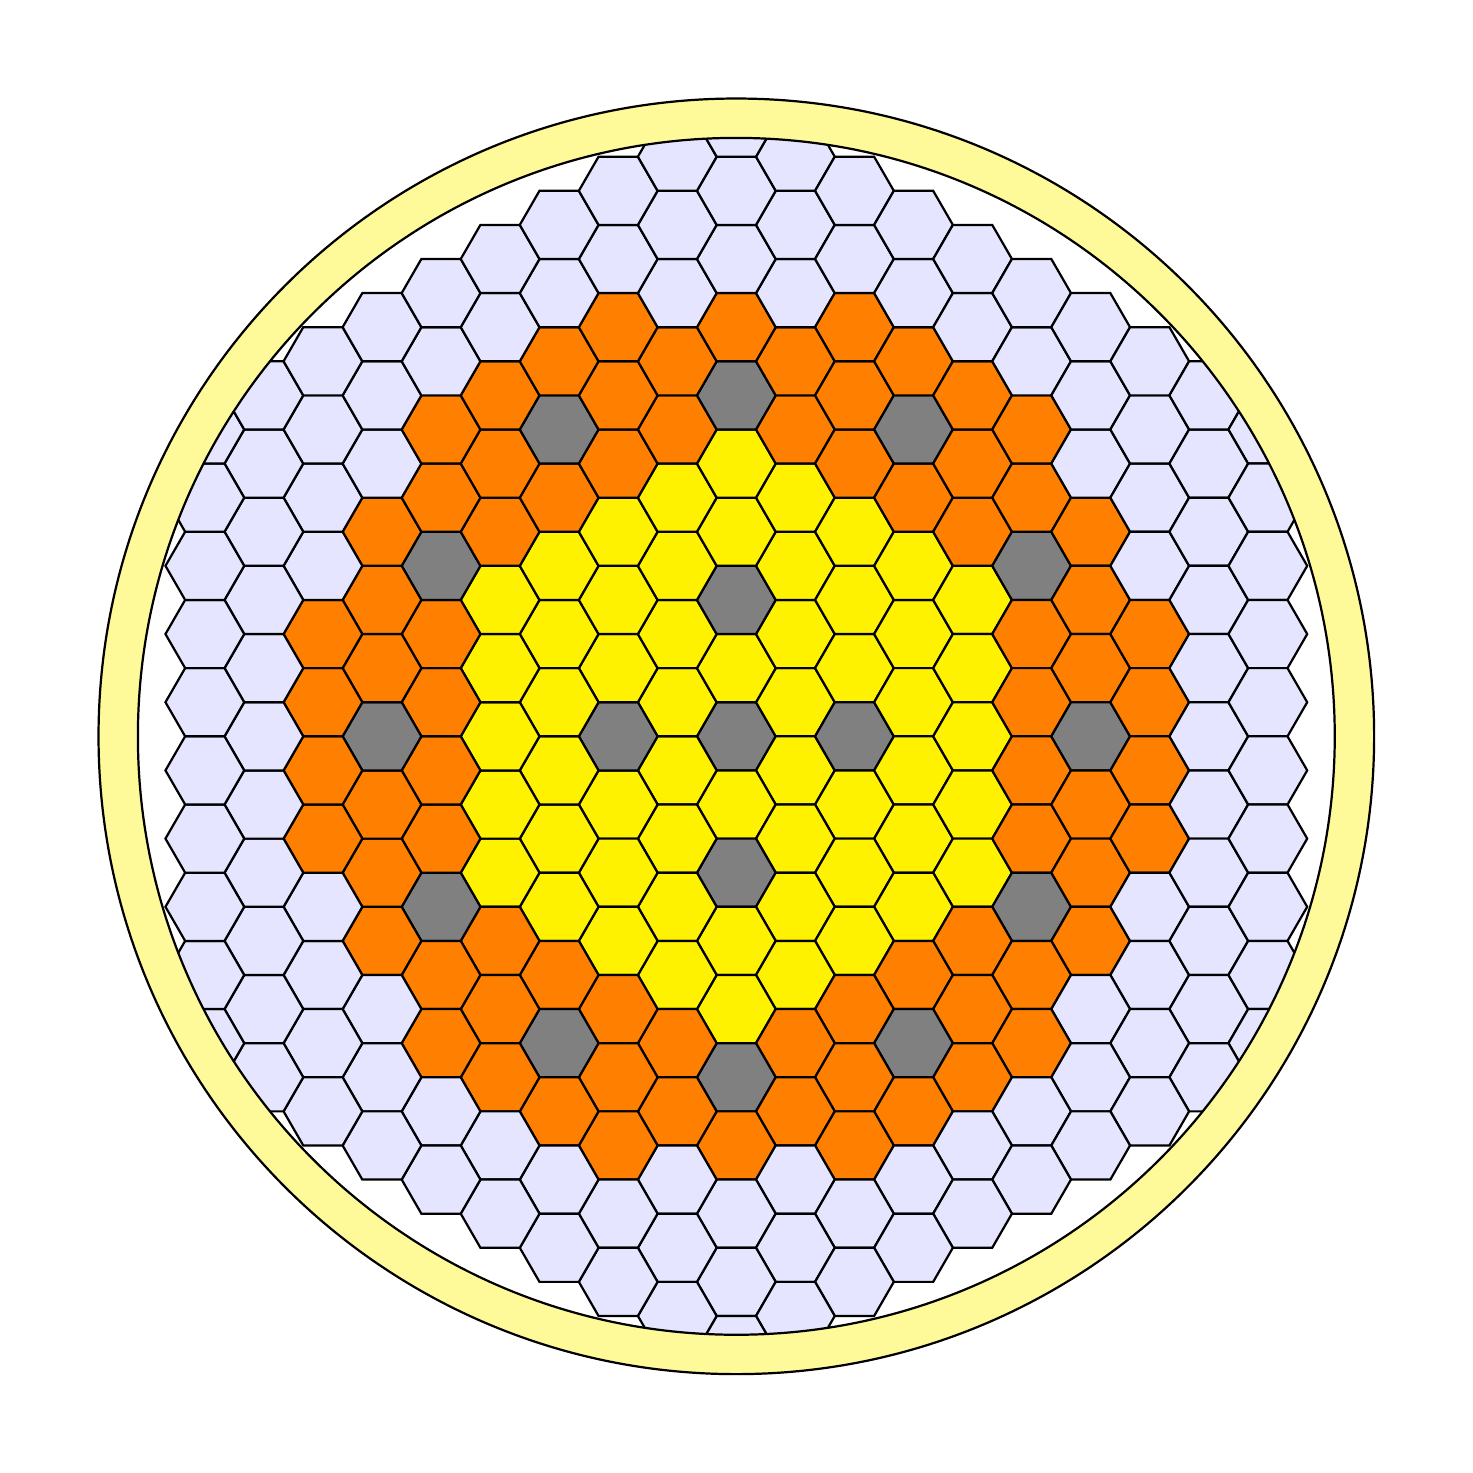
\begin{tikzpicture}
  %%%%%%%%%%%%%%%%%%%%%%%%%%%%%%%%5
    \node[hexagone=0, fill=gray] at (0,0){};
    \foreach \r in {1,...,1}
      \foreach \t in {0,...,5}
        \foreach[evaluate={\l=int(\r*(\r-1)*3+\r*\t+\u)}] \u in {1,...,\r}
          \scoped[rotate=-\t*60]
            \node[hexagone=\l, fill=yellow] at (0+.75*\u,{0.43301270189*(2*\r-\u)}){};
            
   \foreach \r in {2,...,2}
      \foreach \t in {0,...,5}
        \foreach[evaluate={\l=int(\r*(\r-1)*3+\r*\t+\u)}] \u in {1,...,\r}
        \ifthenelse{\l=9 \OR \l=12 \OR \l=15 \OR \l=18}{\def\mycolor{gray}}{\def\mycolor{yellow}}
          \scoped[rotate=-\t*60]
            \node[hexagone=\l, fill=\mycolor] at (0+.75*\u,{0.43301270189*(2*\r-\u)}){}; 
            
            \foreach \r in {3,...,4}
      \foreach \t in {0,...,5}
        \foreach[evaluate={\l=int(\r*(\r-1)*3+\r*\t+\u)}] \u in {1,...,\r}
   %     \ifthenelse{\l=9 \OR \l=12 \OR \l=15 \OR \l=18}{\def\mycolor{violet}}{\def\mycolor{yellow}}
          \def\mycolor{yellow}
          \scoped[rotate=-\t*60]
            \node[hexagone=\l, fill=\mycolor] at (0+.75*\u,{0.43301270189*(2*\r-\u)}){};
            
            
           
         \foreach \r in {5,...,6}
      \foreach \t in {0,...,5}
        \foreach[evaluate={\l=int(\r*(\r-1)*3+\r*\t+\u)}] \u in {1,...,\r}
      \ifthenelse{\l=90 \OR \l=85 \OR \l=80 \OR \l=75 \OR \l=70 \OR \l=65 \OR \l=123 \OR \l=117 \OR \l=111 \OR \l=105 \OR \l=99 \OR \l=93}{\def\mycolor{gray}}{\def\mycolor{orange}}
          \scoped[rotate=-\t*60]
            \node[hexagone=\l, fill=\mycolor] at (0+.75*\u,{0.43301270189*(2*\r-\u)}){};
          
   
   \foreach \r in {7,...,7}
      \foreach \t in {0,...,5}
        \foreach[evaluate={\l=int(\r*(\r-1)*3+\r*\t+\u)}] \u in {1,...,\r}
      \ifthenelse{\l=132 \OR \l=133 \OR \l=134 \OR \l=139 \OR \l=140 \OR \l=141 \OR \l=146 \OR \l=147 \OR \l=148 \OR \l=153 \OR \l=154 \OR \l=155 \OR \l=160 \OR \l=161 \OR \l=162 \OR \l=167 \OR \l=168 \OR \l=127}{\def\mycolor{blue!10}}{\def\mycolor{orange}}
          \scoped[rotate=-\t*60]
            \node[hexagone=\l, fill=\mycolor] at (0+.75*\u,{0.43301270189*(2*\r-\u)}){};
            
            \foreach \r in {8,...,9}
      \foreach \t in {0,...,5}
        \foreach[evaluate={\l=int(\r*(\r-1)*3+\r*\t+\u)}] \u in {1,...,\r}
    %  \ifthenelse{\l=132 \OR \l=133 \OR \l=134 \OR \l=139 \OR \l=140 \OR \l=141 \OR \l=146 \OR \l=147 \OR \l=148 \OR \l=153 \OR \l=154 \OR \l=155 \OR \l=160 \OR \l=161 \OR \l=162 \OR \l=167 \OR \l=168 \OR \l=127}{\def\mycolor{blue!10}}{\def\mycolor{red}}
    \def\mycolor{blue!10}
          \scoped[rotate=-\t*60]
            \node[hexagone=\l, fill=\mycolor] at (0+.75*\u,{0.43301270189*(2*\r-\u)}){};
   
   
  \fill[white,even odd rule] (0,0) circle (9) (0,0) circle (8.1);
  \fill[yellow!40,even odd rule] (0,0) circle (8.1) (0,0) circle (7.6);
  \draw[black,thick] (0, 0) circle (8.1);
  \draw[black,thick] (0, 0) circle (7.6);
   
   

  \end{tikzpicture}
\end{document}